\chapter{Použíté technológie}
\label{chap:pouzite-techologie}
Ako už názov tejto kapitoly napovedá, kapitola predstavuje a popisuje technológie, ktoré boli vybrané v rámci návrhu a následne použité pri samotnej programovej implementácii práce. Celá implementácia, ako aj samotná kapitola, je rozdelená do logických celkov. Podľa týchto celkov bolo potrebné vybrať vhodný programovací jazyk, poprípade aplikačný rámec, pre serverovú časť (aplikačné rozhranie), klientskú časť (aplikácia) a zároveň samotnú databázu.

%%%%%%%%%%%%%%%%%%%%%%%%%%%%%%%%%%%%%%%%%%%%%%%%%%%%%%%%%%%%%%
\section{Klientská časť - aplikácia}
Klientskou časťou je v prípade tejto práce označená samotná hybridná mobilná aplikácia, poprípade aplikácia spustiteľná na desktopovom zariadení. Hybridný prístup k tvorbe aplikácie bol zvolený namiesto klasického natívneho prístupu z dôvodu, že takto vytvorené aplikácie sú vysoko multiplatformné v zmysle, že ich stačí naprogramovať raz a už iba s minimálnym zásahom do kódu pobežia takmer na väčšine bežných operačných systémov. Bol zvolený hybridný aplikačný rámec Ionic verzia 2, ktorý je postavený na programovacom jazyku Typescript (nadmnožina jazyka Javascript) a na aplikačnom rámci Angular2. Typescript sa v rámci Ionic používa na logiku aplikácie. Pre vizuál aplikácie sa používa klasické HTML a CSS, alebo preprocesor SCSS. Táto práca je zameraná na  platformu Android a platformu Windows. Platformu android je možné pokryť pomocou technológie Apache Cordova, Windows zase pomocou technológie Electron. 
\begin{itemize}
    \item \textbf{HTML -} Hyper Text Markup Language je momentálne najpoužívanejší značkovací jazyk pre tvorbu webových stránok. HTML pre popis dokumentu používa značkovacie tagy, ktoré hovoria danému programu, internetovému prehliadaču, ako má daný dokument štruktúrovať. Originálne bol tento jazyk vyvinutý pre popis štruktúry dokumentov, hlavne nadpisov, paragrafov, zoznamov, ktoré sa zdieľali medzi inštitúciami a vedeckými pracovníkmi. Postupom času sa avšak z HTML stal celosvetovo rozšírený štandard pre popis štruktúry webových stránok. V minulosti sa HTML používalo nielen pre popis štruktúry, ale aj pre popis jeho výzoru. V súčastnosti sa výzor webových stránok definuje pomocou CSS. \cite{fswG1WVQQnoCa64c}
    \item \textbf{CSS -} Cascading Style Sheet je jednoduchý dizajnérsky jazyk, ktorý popisuje ako budú dané HTML tagy zobrazené na obrazovke počítača, papieri, alebo inom médiu. Medzi hlavné výhody CSS patrí to, že šetrí čas, pretože štýl napísaný v CSS je možné potom ďalej používať na iné webové stránky a zároveň sa zrýchľuje načítanie stránok, keďže sa štýl nedefinuje väčšinou po jednom tagu, alebo po celej triede tagov. V priebehu rokov sa z CSS, tak ako to bolo aj s HTML, stal štandard pre webové stránky a podporujú ho všetky moderné webové prehliadače. \cite{VNZJ2nmvOm16rWtR}
    \item \textbf{SCSS -} Syntactically Awesome Stylesheet, je CSS preprocesor, ktorý rozširuje bežné CSS o celú radu vylepšení. Za zmienku stoja napríklad premenné, zanorovanie pravidiel, importy. To má za následok, že kód je oveľa viac organizovaný, prehľadnejší, rozsahovo menší a je možné dosiahnuť netriviálnych cieľov oveľa jednoduchšie. Jedná sa v podstate o nadmonžinu CSS. Varianta syntakticky viac podobná klasickému CSS sa nazýva SCSS (Sassy CSS). \cite{SIWRi1jHe5vClhda}
    \item \textbf{Javascript -} je interpretovaný objektovo-orientovaný programovací jazyk, ktorý je známi predovšetkým ako skriptovací jazyk používaný na webových stránkach. V kontexte webových stránok sa používa predovšetkým pre dynamickú manipuláciu, ako napríklad odozvy na rôzne udalosti, animácie a iné. Je spúšťaný webovým prehliadačom. V súčastnosti sa rozširuje aj mimo klientskú stranu webu a je ho možné vidieť ako serverové riešenie v podobe stále viac populárneho Node.js. Je založený na vytváraní prototypov. Podporuje imperatívne, ale aj funkcionálne programovanie. \cite{mpahm68E0P8GyL7C}
    \item \textbf{Typescript -} Ako aplikácia napísaná v Javascripte rastie, tak začína byť neprehľadná a ťažko udržovateľná. Z toho dôvodu Microsoft vyvinul Typescript. Typescript je vlastne nadmnožina Javascriptu, ktorá nezahŕňa iba samotný jazyk, ale aj početnú sadu nástrojov. Všetok kód napísaný v Typescripte sa transpiluje do čistého Javascriptu. Typescript rozširuje obyčajný Javascript o silné statické typovanie a je plne objektovo orientovaný (je možné použiť dedičnosť, triedy, rozhrania a iné veci typické pre čisto objektovo orientované jazyky). V neposlednom rade je v ňom možné používať všetky bežné Javascriptové knižnice. \cite{f7jKojjQlPsziQuS}
    \item \textbf{Angular2 -} je Typescriptový aplikačný rámec pre tvorbu webových tzv. Single Page aplikácií. Je vyvinutý týmom z Googlu, ktorý pracoval aj na originálnom AngularJS. Aj keď Angular2 a AngularJS majú podobné princípy, prakticky ide o dva odlišné aplikačné rámce. Tento rámec bol prvý krát predstavený v roku 2014. Jeho myšlienka je založená na tvorbe znovupoužiteľných komponentov a v podstate využíva o Model Controler View architektúru, ktorú je ale možné vymeniť napríklad za architektúru Redux, známu hlavne z Facebook rámca React. \cite{oHlcq3e3366Aa2oa}
    
    Single page aplikácie sú webové aplikácie, ktoré používajú väčšinou server iba ako zdroj a úložisko dát. Získané dáta sú následne vykresľované na klientovi pomocou Javascriptu. Pri prvom príchode na takúto stránku sa najprv stiahnu potrebné Javascriptové súbory a základná kostra HTML. Následne sa vykonajú operácie, ktoré určia, čo sa má zobraziť. Podľa toho čo sa má zobraziť je asynchrónnym dotazom (AJAX) na server požiadané o dáta, ktoré prídu v odpovedi typicky vo formáte JSON. Pri ďalšej interakcií so stránkou sa robia vždy len dotazy na samotný obsah. Server je v prípade takýchto webových stránok pasovaný iba do jednoduchého rozhrania, ktoré spracováva požiadavky z klienta a poprípade získava a ukladá dáta. \cite{Jahoda2015}
    \begin{figure}[h]
        \centering
        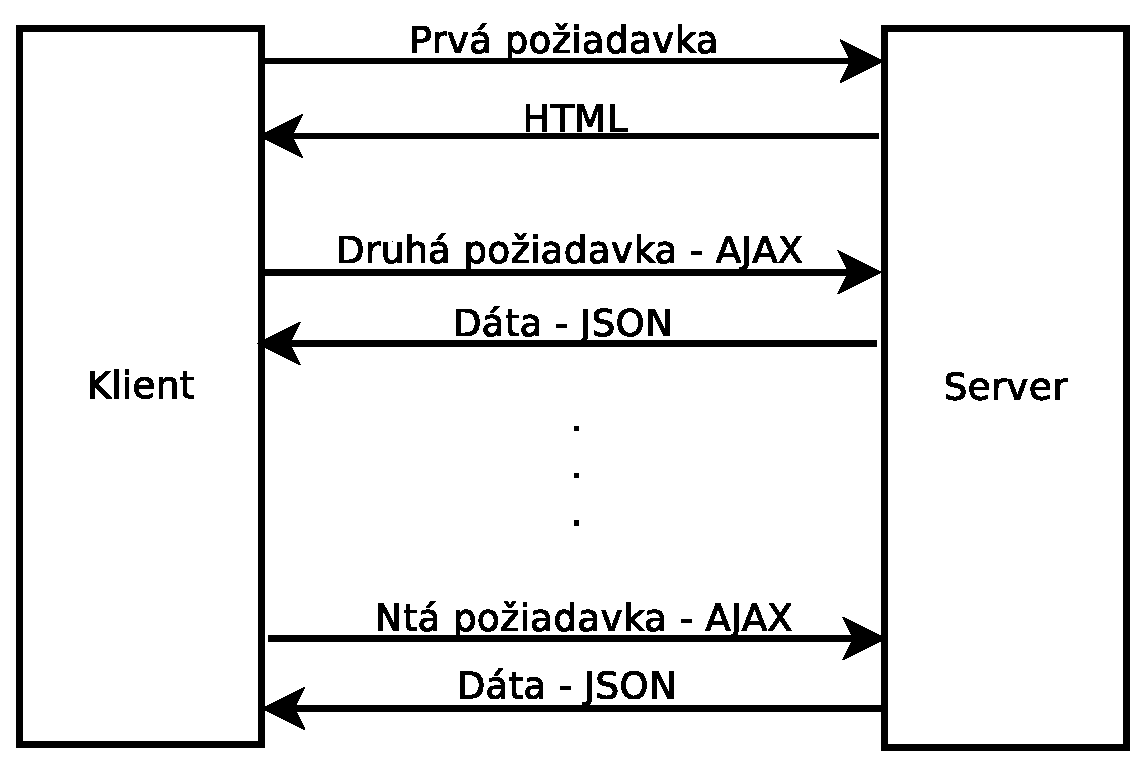
\includegraphics[scale=0.5]{fig/spa.eps}
        \caption{Klient-server komunikácia v Single page aplikácii.}
        \label{fig:spa}
    \end{figure}
    \pagebreak
    \item \textbf{Cordova -} je rámec, ktorý zabalí HTML, CSS a Javascript aplikáciu do natívneho kontaineru, WebView, ktorý vo výsledku vyzerá a chová sa ako bežná natívna aplikácia. Kontainer dokáže pristupovať k funkciám zariadenia vďaka natívnym zásuvným modulom a Javascriptovému aplikačnému rozhraniu. Cordova podporuje celú škálu platforiem od Android, cez iOS, až po Windows Phone. Projekt bol najprv vytvorený firmou Nitobi, ktorá bola v roku 2011 kúpená známou firmou Adobe Systems. Adobe Systems následne uvoľnila kód Cordovy. \cite{DVKuXjtaapUpB12M}
    \begin{figure}[h]
      \centering
      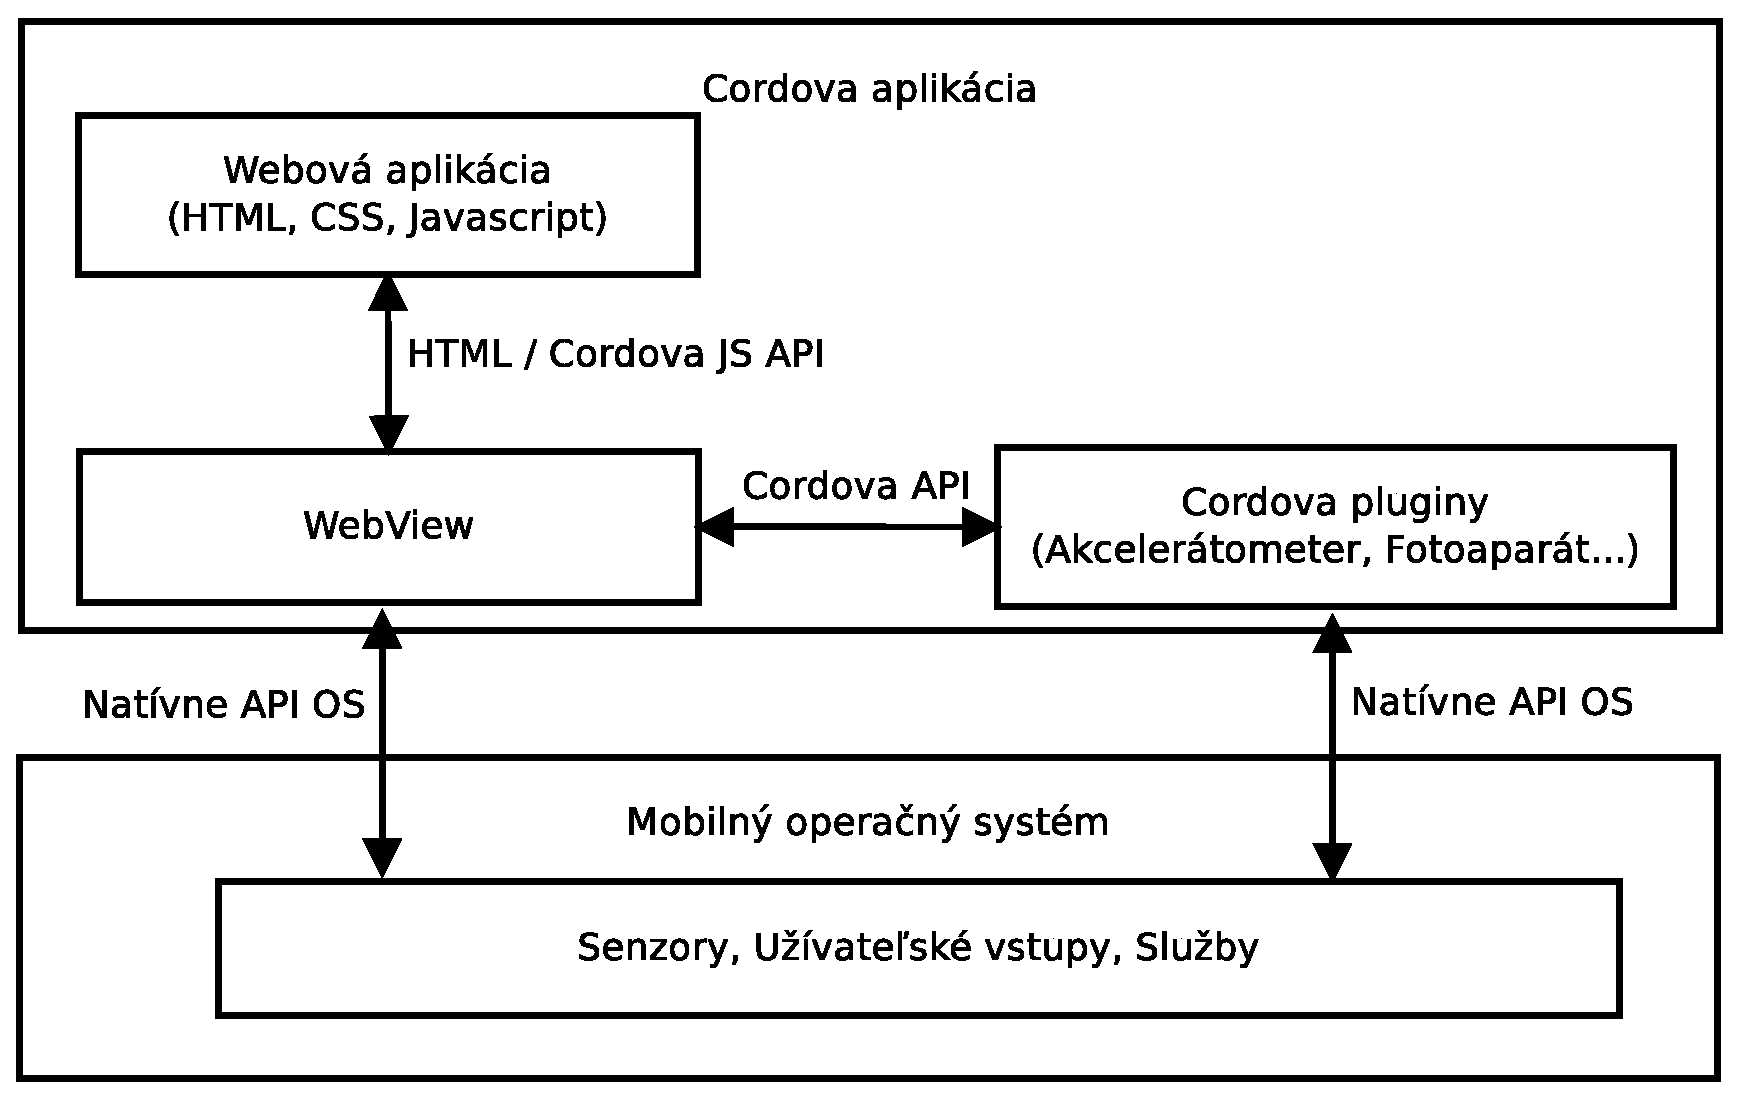
\includegraphics[scale=0.35]{fig/cordova.eps}
      \caption{Architektúra aplikácie vytvorenej pomocou Cordova technológie.}
      \label{fig:cordova}
    \end{figure}
    \item \textbf{Ionic2 -} je kompletné SDK pre vývoj hybridných mobilných aplikácií. Celý aplikačný rámec je postavený na Angular2 a  rozširuje ho o ďalšie komponenty a funkcionalitu typickú pre mobilné zariadenia. Pomocou Cordova zásuvným modulom a ich implementácií v tomto rámci je možné tiež pristupovať k natívnym funkciám zariadenia. \cite{HiUt1XS9KvN1fiB5}
    
    Hybridné mobilné aplikácie sú aplikácie, ktoré na prvý pohľad vypadajú ako natívne aplikácie, avšak ich programovanie prebiehalo väčšinou pomocou webových technológií s následným zabalením pomocou technológie Cordova, alebo inej podobnej. Medzi  najväčšiu výhodu takéhoto prístupu patrí to, že aplikáciu stačí napísať iba raz a potom ju je možné už iba s drobnými zmenami vydávať na rôzne mobilné platformy.\cite{0QSW9GoG0OTJ7FKM}
    \item \textbf{Electron -} je knižnica vyvinutá GitHubom pre tvorbu multiplatformných desktopových aplikácií pomocou webových technológií, ktoré už boli popísané. Electron je ponúkaný pod licenciou MIT a má otvorený kód. Využíva kombináciu technológie Chromium a Node.js, ktoré zabalí spolu s webovou aplikáciou do jednej výslednej aplikácie. Takúto výslednú aplikáciu je možné spúšťať na platforme Windows, Mac a aj Linux. K natívnym funkciám operačného systému je možné pristupovať, tak ako v prípade Cordovy, pomoocu natívnych aplikačných rozhraní. \cite{hBGbGXxiU66nJt51}
    \begin{figure}[h]
      \centering
      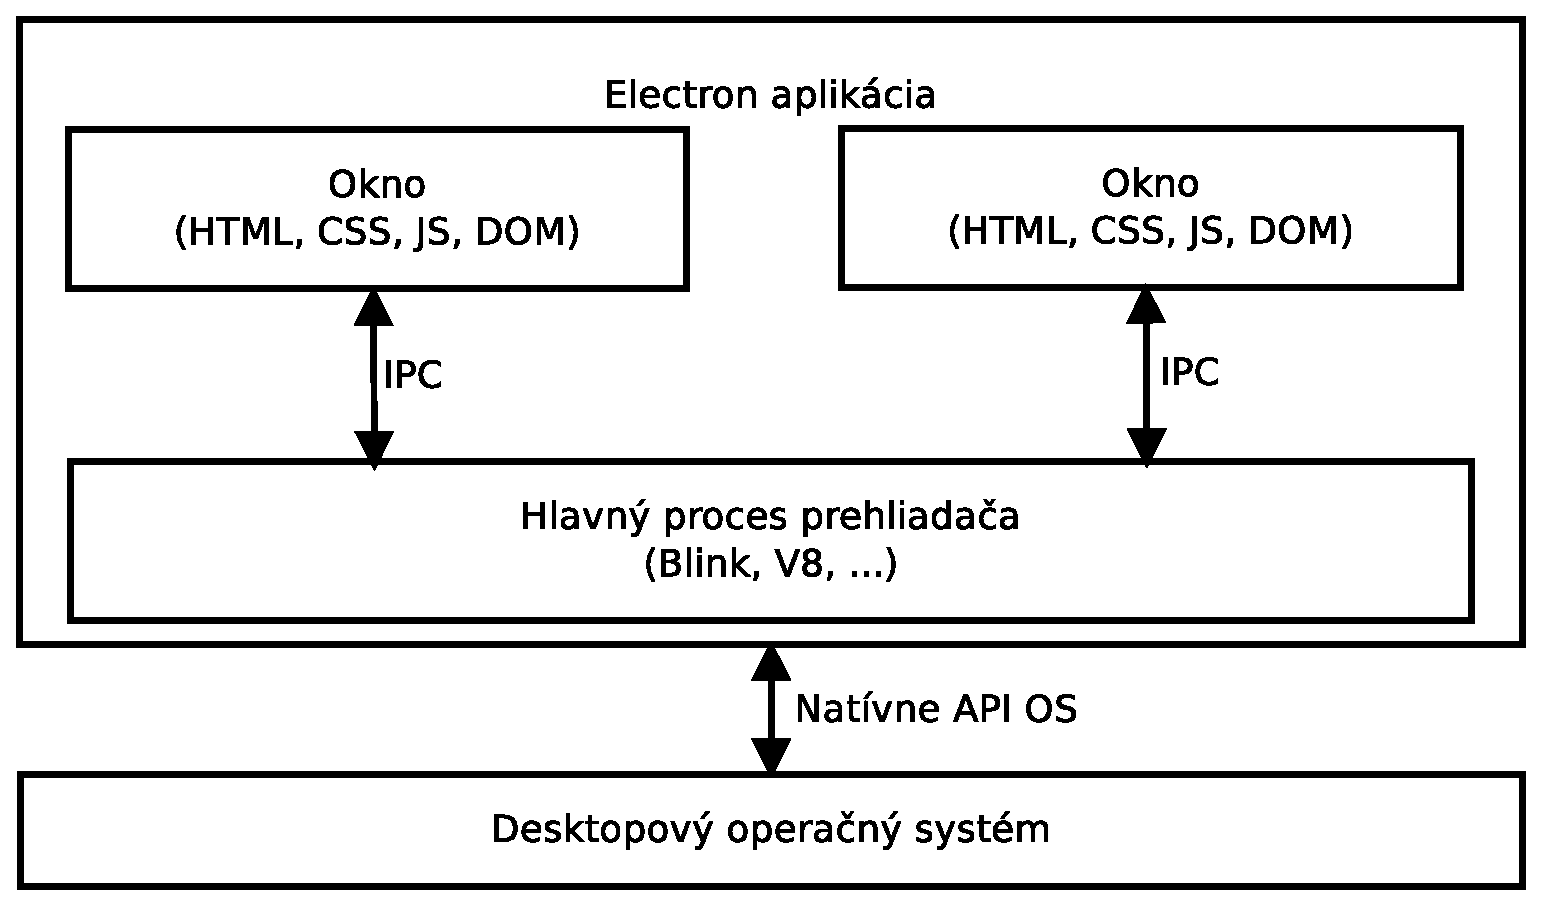
\includegraphics[scale=0.40]{fig/electron.eps}
      \caption{Architektúra aplikácie vytvorenej pomocou Electron rámca.}
      \label{fig:electron}
    \end{figure}
\end{itemize}

%%%%%%%%%%%%%%%%%%%%%%%%%%%%%%%%%%%%%%%%%%%%%%%%%%%%%%%%%%%%%%
\section{Serverová časť - aplikačné rozhranie}
Serverová časť pokrýva všetky operácie, ktoré sa nevykonávajú priamo v zariadení, ale vykonávajú sa vzdialene na strane serveru. Medzi takéto operácie patrí napríklad ukladanie dát do databáze, autentifikácia, autorizácia užívateľa, alebo samotná práca so snímkom chronickej rany. Serverová časť v tejto práci tvorí vzdialené aplikačné rozhranie. Je tvorená pomocou skriptovacieho jazyka Python, za pomoci aplikačného rámca Flask. Flask vo svojom jadre dodržiava princípy REST a je vďaka tomu možné jednoducho navrhnúť plne funkčné RESTful aplikačné rozhranie, s ktorým v tejto práci priamo komunikuje klientská aplikácia. Pre spracovanie obrazu, konkrétne samotných fotiek chronických rán, bola vybraná Python implementácia populárnej knižnice na spracovanie obrazu zvaná OpenCV.
\begin{itemize}
    \item \textbf{REST -} Representational state transfer je súbor niekoľkých prísnych, ale jasne definovaných pravidiel pre návrh architektúry distribuovaného systému, hlavne rozhrania medzi jednotlivými komponentami, poprípade serverovou a klientskou časťou. Základným stavebným kameňom RESTu je zdroj. Zdroj môže byť čokoľvek, napríklad konkrétny objekt v databáze, dokument a podobne. Základným pravidlom je, že každý objekt musí mať svoju URL. Klient nikdy nevidí zdroj priamo, ale vždy iba jeden z jeho obrazov, ktorý je nazývaný reprezentácia. Reprezentácia je strojovo čitateľná reprezentácia aktuálneho stavu zdroja. Môže to byť obrázok, HTML stránka a podobne. Výber reprezentácie môže byť ovplyvnený klientom pomocou riadiacej informácie, alebo serverom na základe klasifikácie klienta. Samotná komunikácia cez REST je bezstavová, čo znamená, že každý požiadavok obsahuje všetky informácie potrebné k jeho vykonaniu. REST definuje 4 základné operácie: POST pre vytváranie, GET pre získavanie, PUT pre zmenu a DELETE pre vymazávanie. \cite{54r2mhdAeuyxzZPp}
    \item \textbf{Python -} je open source objektovo-orientovaný vysokoúrovňový skriptovaci jazyk, ktorý vytvoril Guido van Rossum v rokoch 1985-1990. Kód Pythonu spadá pod licenciu GNU General Public License. Python je interpretovaný a teda nie je nutné programy v ňom napísané prekladať. Programy sú namiesto prekladu priamo vykonávané interpreterom. Okrem toho je taktiež interaktívny. To znamená, že užívateľ môže priamo interagovať s interpreterom a písať programy aj týmto spôsobom. Ďalšou nespornou výhodou Pythonu je to, že je rozšíriteľný a nízko-úrovňové moduly sa dajú písať v programovacom jazyku C. Vďaka tomu môže byť dosiahnuté lepšej efektivity. \cite{CCnsn576LIGBCH2C}
    
    Python bol zvolený najmä kvôli tomu, že je pomerne rozšírený, bežne sa používa na serverovú časť webových informačných systémov, má na výber z veľkého množstva intuitívnych aplikačných rámcov, dobre si rozumie s relačnými, ale aj s NoQSL databázami a v neposlednom rade je preň dostupná implementácia OpenCV.
    \item \textbf{Flask -} je aplikačný mini rámec, ktorý je napísaný v programovacom jazyku Python. Slúži pre vývoj webových aplikácií, alebo vo všeobecnosti serverových častí informačných systémov, poprípade aplikačných rozhraní. V základe má k dispozícií iba funkcie s prácou pre URL, HTTP a šablónami. Z toho plynie, že je jednoduchý na osvojenie a pre účely tejto práce úplne postačuje. \cite{YNlrXY2RKWca3gk8}
    \item \textbf{OpenCV -} je knižnica počítačového videnia. Je napísaná v jazyku C a C++ a je možné ju použiť na všetkých bežných aktuálnych platformách. Rozhranie je dostupné pre Python, Java, Ruby a ostatné bežné programovacie jazyky. OpenCV bolo navrhnuté pre výpočtovú efektivitu so silným dôrazom na aplikácie bežiace v reálnom čase. Optimalizácie knižnice boli vykonávané na všetkých úrovniach, od algoritmov až po viac jadrové inštrukcie procesorov. Hlavným cieľom je ponúknuť jednoduchú infraštruktúru počítačového videnia, ktorá by pomáhala ľuďom tvoriť zložitejšie aplikácie oveľa rýchlejšie a jednoduchšie. Samotná knižnica obsahuje viac ako 500 funkcií, pokrývajúce rôzne odvetvia vedy. OpenCV v sebe obsahuje okrem svojej samotnej implementácie aj pod-knižnice pre strojové učenie. keďže počítačové videnie a strojové učenie spolu úzko súvisia. Pod-knižnice sa z veľkej časti orientujú na rozpoznávanie vzorov a rozdeľovanie do zhlukov. \cite{Bradskic2008}
\end{itemize}

%%%%%%%%%%%%%%%%%%%%%%%%%%%%%%%%%%%%%%%%%%%%%%%%%%%%%%%%%%%%%%
\section{Databázová časť}
Pre uchovanie dát na strane serveru bola zvolená možnosť uloženia do databáze. Táto možnosť bola zvolená kvôli tomu, že manipulácia s dátami je pomerne rýchla, keďže sa do pamäte neukladá celá databáza, ale iba jej požadovaná časť. Okrem toho, pre získanie dát sa dá použiť pokročilejší dotazovací jazyk a je podporovaný prístup viacerých užívateľov súčasne. 

Ako databáza bol zvolený typický zástupca NoSQL databáz menom MongoDB, ktorý je vyvíjaný MongoDB industries a má otvorený zdrojový kód. Dáta ukladá v štruktúre podobnej JSON dokumentom, a to v štruktúre Binary JSON, ktorý samotný JSON obohacuje o ďalšie typy. Súvisiace informácie sú uložené spolu pre rýchly dotazovací prístup pomocou MongoDB dotazovacieho jazyka. Používa dynamické schémy, to znamená, že záznamy nemajú pevne danú štruktúru a v priebehu sa táto štruktúra môže meniť. Pomocou tohoto dátového modelu je možné reprezentovať hierarchické vzťahy a ukladať polia a iné komplexnejšie dátové štruktúry. MongoDB dbá na to, aby bola zabezpečená vysoká dostupnosť a škálovateľnosť. Nespornou výhodou NoSQL a konkrétne MongoDB oproti Mysql je, že vývoj aplikácie s MongoDB je jednoduchší, keďže sa dokumenty v databáze prirodzene mapujú do moderných objektovo orientovaných jazykov a odpadá tak objektovo relačné mapovanie objektov. Obrovskou výhodou oproti napríklad MySQL je už spomínaná škálovateľnosť. Samotné MongoDB vyžaduje pre svoje fungovanie iba adresár na uloženie dát a teda môže byť ľahko distribuované spolu s programom. \cite{9egOMsyThyK0MyF2}
\begin{lstlisting}[caption={Ukážka štruktúry NoSQL MongoDB databáze.},captionpos=b]
[
    item1ID: {
	    name: 'MongoDB',
	    description: 'NoSQL'
    },
    item2ID: {
	    name: 'MySQL',
	    description: 'Relational'
    }
]
\end{lstlisting}